% Convert to .eps instructions:
% pdfcrop $2.pdf
% pdftops -f $1 -l $1 -eps "$2-crop.pdf"
% rm  "$2-crop.pdf"
% mv  "$2-crop.eps" $2.eps

\documentclass[tikz,border=5pt]{standalone}
% \documentclass[convert={outext=.eps, command=\unexpanded{pdftops -eps \infile}}]{standalone}

\newcommand{\VAR}{Success}

% COORDINATES

% Preliminaries
\newcommand{\PHIANGLE}{30}   % 0 <  phi  < 45 : Controls left to right rotation
\newcommand{\THETAANGLE}{35} % 0 < theta < 90 : Controls top to bottom rotation
\newcommand{\COSTHETA}{cos(\THETAANGLE)}
\newcommand{\SINTHETA}{sin(\THETAANGLE)}
\newcommand{\COSPHI}{cos(\PHIANGLE)}
\newcommand{\SINPHI}{sin(\PHIANGLE)}
\newcommand{\ORIGINX}{0.0}
\newcommand{\ORIGINY}{0.0}
\newcommand{\DX}{2}
\newcommand{\DY}{2}
\newcommand{\DZ}{2}
\newcommand{\DIAGX}{\DZ*\COSPHI*\SINPHI*\COSTHETA}
\newcommand{\DIAGY}{\DZ*\SINPHI*\COSPHI*\SINTHETA}

% CELL CENTER
\newcommand{\CCX}{\ORIGINX}
\newcommand{\CCY}{\ORIGINY}

% FACES
\newcommand{\XBFACEX}{\CCX-.5*\DX}
\newcommand{\XTFACEX}{\CCX+.5*\DX}
\newcommand{\YBFACEX}{\CCX}
\newcommand{\YTFACEX}{\CCX}
\newcommand{\ZBFACEX}{\CCX+.5*\DIAGX}
\newcommand{\ZTFACEX}{\CCX-.5*\DIAGX}

\newcommand{\XBFACEY}{\CCY}
\newcommand{\XTFACEY}{\CCY}
\newcommand{\YBFACEY}{\CCY-.5*\DY}
\newcommand{\YTFACEY}{\CCY+.5*\DY}
\newcommand{\ZBFACEY}{\CCY+.5*\DIAGY}
\newcommand{\ZTFACEY}{\CCY-.5*\DIAGY}

% EDGES
\newcommand{\XEDGEAX}{\ZBFACEX} % Edge 1
\newcommand{\XEDGEBX}{\ZTFACEX} % Edge 1
\newcommand{\XEDGECX}{\ZBFACEX} % Edge 1
\newcommand{\XEDGEDX}{\ZTFACEX} % Edge 1
\newcommand{\YEDGEAX}{\ZBFACEX-.5*\DX} % Edge 1
\newcommand{\YEDGEBX}{\ZTFACEX-.5*\DX} % Edge 1
\newcommand{\YEDGECX}{\ZBFACEX+.5*\DX} % Edge 1
\newcommand{\YEDGEDX}{\ZTFACEX+.5*\DX} % Edge 1
\newcommand{\ZEDGEAX}{\XBFACEX} % Edge 1
\newcommand{\ZEDGEBX}{\XTFACEX} % Edge 1
\newcommand{\ZEDGECX}{\XBFACEX} % Edge 1
\newcommand{\ZEDGEDX}{\XTFACEX} % Edge 1

\newcommand{\XEDGEAY}{\ZBFACEY-.5*\DY} % Edge 1
\newcommand{\XEDGEBY}{\ZTFACEY-.5*\DY} % Edge 1
\newcommand{\XEDGECY}{\ZBFACEY+.5*\DY} % Edge 1
\newcommand{\XEDGEDY}{\ZTFACEY+.5*\DY} % Edge 1
\newcommand{\YEDGEAY}{\ZBFACEY} % Edge 1
\newcommand{\YEDGEBY}{\ZTFACEY} % Edge 1
\newcommand{\YEDGECY}{\ZBFACEY} % Edge 1
\newcommand{\YEDGEDY}{\ZTFACEY} % Edge 1
\newcommand{\ZEDGEAY}{\XBFACEY-.5*\DZ} % Edge 1
\newcommand{\ZEDGEBY}{\XTFACEY-.5*\DZ} % Edge 1
\newcommand{\ZEDGECY}{\XBFACEY+.5*\DZ} % Edge 1
\newcommand{\ZEDGEDY}{\XTFACEY+.5*\DZ} % Edge 1

% NODES
\newcommand{\NODEAX}{\XEDGEAX-0.5*\DX}
\newcommand{\NODEBX}{\XEDGEAX+0.5*\DX}
\newcommand{\NODECX}{\XEDGECX-0.5*\DX}
\newcommand{\NODEDX}{\XEDGECX+0.5*\DX}
\newcommand{\NODEEX}{\XEDGEBX-0.5*\DX}
\newcommand{\NODEFX}{\XEDGEBX+0.5*\DX}
\newcommand{\NODEGX}{\XEDGEDX-0.5*\DX}
\newcommand{\NODEHX}{\XEDGEDX+0.5*\DX}

\newcommand{\NODEAY}{\XEDGEAY}
\newcommand{\NODEBY}{\XEDGEAY}
\newcommand{\NODECY}{\XEDGECY}
\newcommand{\NODEDY}{\XEDGECY}
\newcommand{\NODEEY}{\XEDGEBY}
\newcommand{\NODEFY}{\XEDGEBY}
\newcommand{\NODEGY}{\XEDGEDY}
\newcommand{\NODEHY}{\XEDGEDY}
 % For local use
\input{\rootdir/includes/margins/zero_margins.tex}


 % For local use
\setlength{\voffset}{-1in}
\setlength{\hoffset}{-1in}
\usetikzlibrary{positioning}
\usetikzlibrary{shapes.geometric,calc}
% \usepackage{tikzexternal}
% \tikzexternalize

% Equation font size
\newcommand{\EQS}{\Huge}

% Length of arrowed parts
\newcommand{\arrowL}{0.4}
\newcommand{\coordL}{0.2}

% Thickness of lines
\newcommand{\w}{2}
\newcommand{\wCrissCross}{\w/2}
\newcommand{\wCoord}{\w}
\newcommand{\wArr}{5}
\newcommand{\s}{4.8} % New

% Arrow head type and direction
\newcommand{\arrL}{stealth-}
\newcommand{\arrR}{-stealth}
\newcommand{\arrLR}{-stealth-}

\begin{document}
\MOONSTITLE
\pagenumbering{gobble}
\noindent

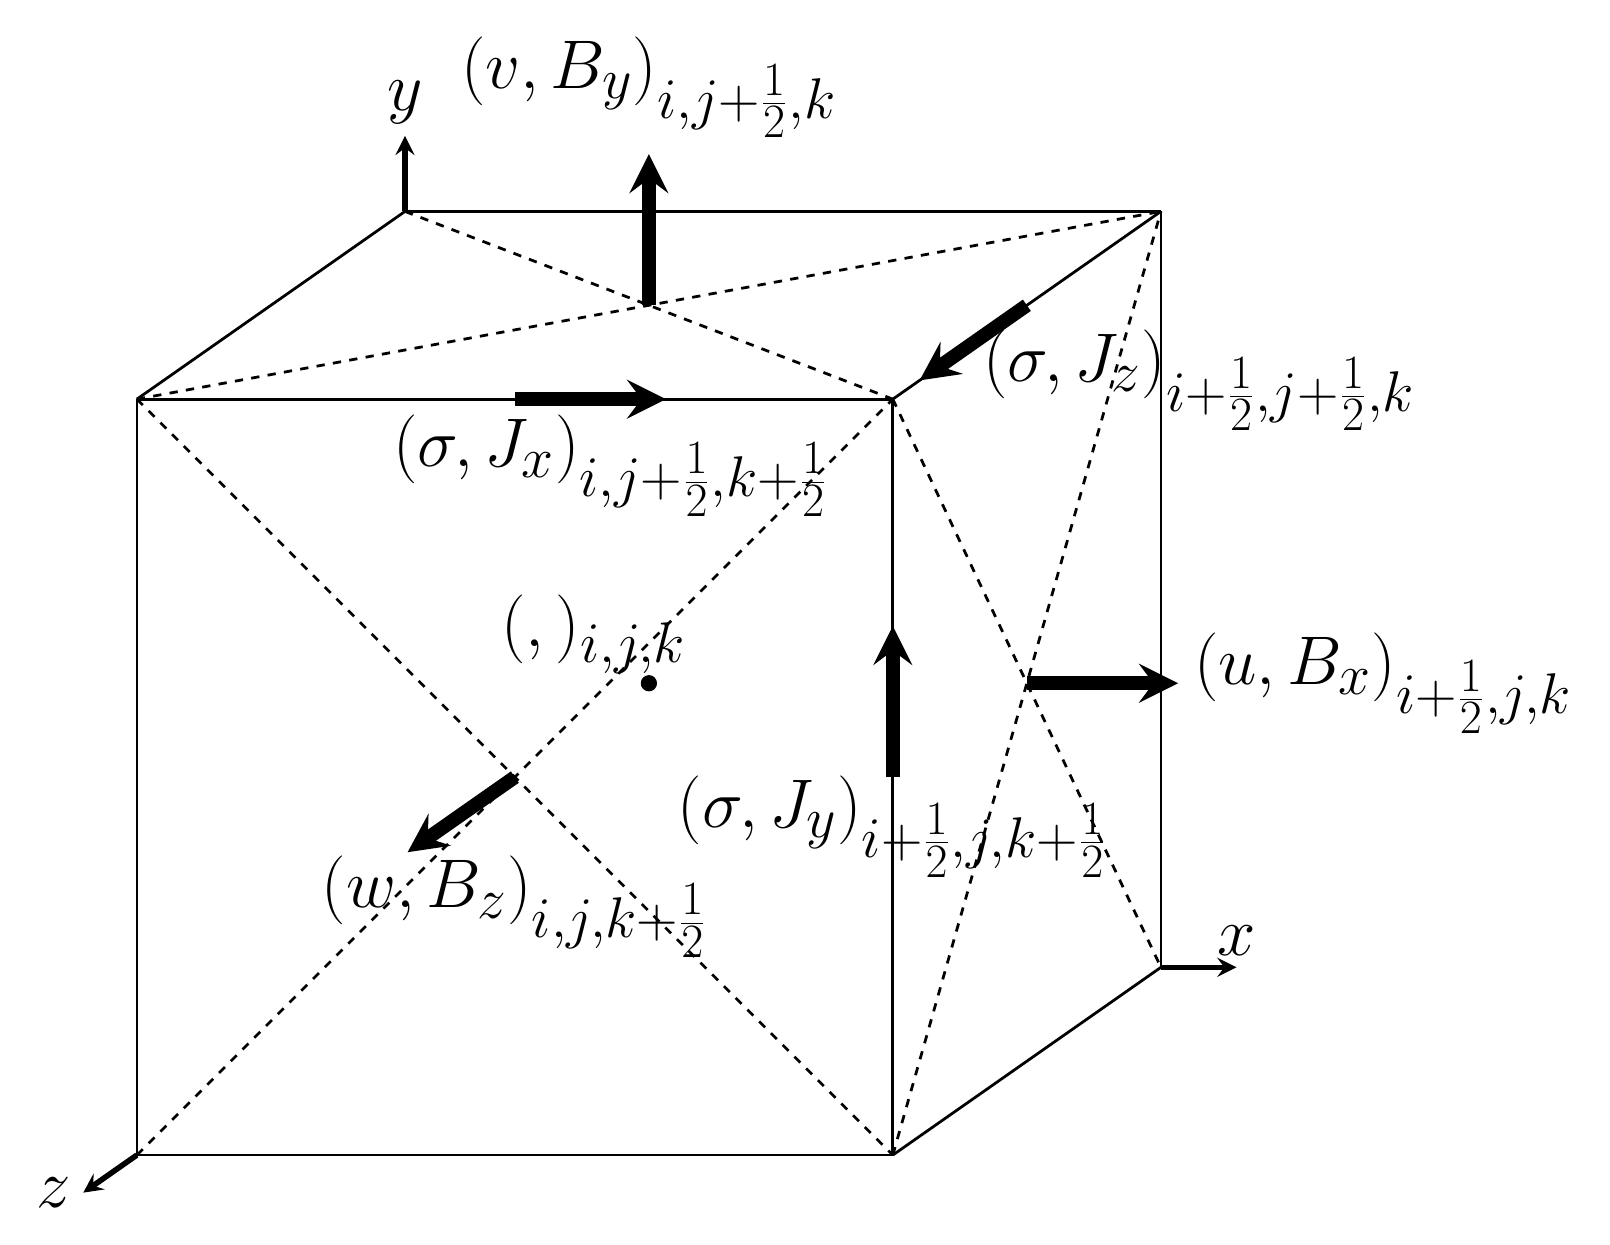
\begin{tikzpicture}[scale=\s]
\tikzstyle{every node}=[font=\LARGE]
% Node lines
	% \draw[line width=1,dashed] ({\NODEAX},{\NODEAY}) -- ({\NODEBX},{\NODEBY});
	\draw[line width=1] ({\NODECX},{\NODECY}) -- ({\NODEDX},{\NODEDY});
	\draw[line width=1] ({\NODEEX},{\NODEEY}) -- ({\NODEFX},{\NODEFY});
	\draw[line width=1] ({\NODEGX},{\NODEGY}) -- ({\NODEHX},{\NODEHY});

	% \draw[line width=1,dashed] ({\NODEAX},{\NODEAY}) -- ({\NODEEX},{\NODEEY});
	\draw[line width=1] ({\NODEBX},{\NODEBY}) -- ({\NODEFX},{\NODEFY});
	\draw[line width=1] ({\NODECX},{\NODECY}) -- ({\NODEGX},{\NODEGY});
	\draw[line width=1] ({\NODEDX},{\NODEDY}) -- ({\NODEHX},{\NODEHY});

	% \draw[line width=1,dashed] ({\NODEAX},{\NODEAY}) -- ({\NODECX},{\NODECY});
	\draw[line width=1] ({\NODEBX},{\NODEBY}) -- ({\NODEDX},{\NODEDY});
	\draw[line width=1] ({\NODEEX},{\NODEEY}) -- ({\NODEGX},{\NODEGY});
	\draw[line width=1] ({\NODEFX},{\NODEFY}) -- ({\NODEHX},{\NODEHY});

% Criss-cross lines (Sergey's request)
	\draw[line width=\wCrissCross,dashed] ({\NODEFX},{\NODEFY}) -- ({\NODEDX},{\NODEDY});
	\draw[line width=\wCrissCross,dashed] ({\NODEHX},{\NODEHY}) -- ({\NODEBX},{\NODEBY});
	\draw[line width=\wCrissCross,dashed] ({\NODEGX},{\NODEGY}) -- ({\NODEDX},{\NODEDY});
	\draw[line width=\wCrissCross,dashed] ({\NODECX},{\NODECY}) -- ({\NODEHX},{\NODEHY});
	\draw[line width=\wCrissCross,dashed] ({\NODEEX},{\NODEEY}) -- ({\NODEHX},{\NODEHY});
	\draw[line width=\wCrissCross,dashed] ({\NODEGX},{\NODEGY}) -- ({\NODEFX},{\NODEFY});

% Lines to faces
	% \draw[line width=1] ({\CCX},{\CCY}) -- ++ ({\XTFACEX},{\XTFACEY});
	% \draw[line width=1] ({\CCX},{\CCY}) -- ++ ({\YTFACEX},{\YTFACEY});
	% \draw[line width=1] ({\CCX},{\CCY}) -- ++ ({\ZTFACEX},{\ZTFACEY});

% Face fields:
	\draw[line width=\wArr,\arrR] ({\XTFACEX},{\XTFACEY}) -- ++ ({\arrowL},{0})                        node[anchor=west]  {\EQS $(u,B_x)_{i+\frac{1}{2},j,k}$};
	\draw[line width=\wArr,\arrR] ({\YTFACEX},{\YTFACEY}) -- ++ ({0},{\arrowL})                        node[anchor=south]  {\EQS $(v,B_y)_{i,j+\frac{1}{2},k}$};
	% \draw[line width=\wArr,\arrR] ({\ZTFACEX},{\ZTFACEY}) -- ++ ({-\arrowL*\DIAGX},{-\arrowL*\DIAGY})  node[right=1,anchor=north]  {\EQS $(w,B_z)_{i,j,k+\frac{1}{2}}$};
	% \draw[line width=\wArr,\arrL] ({\ZTFACEX-\arrowL*\DIAGX},{\ZTFACEY-\arrowL*\DIAGY}) -- ++ ({\arrowL*\DIAGX},{\arrowL*\DIAGY})  node[below=2,anchor=north]  {\EQS $(w,B_z)_{i,j,k+\frac{1}{2}}$};
	\draw[line width=\wArr,\arrL] ({\ZTFACEX-\arrowL*\DIAGX},{\ZTFACEY-\arrowL*\DIAGY}) -- ++ ({\arrowL*\DIAGX},{\arrowL*\DIAGY})  node[below=.8,anchor=north]  {\EQS $(w,B_z)_{i,j,k+\frac{1}{2}}$};

% Edge fields:
	% \draw[line width=\wArr,\arrR] ({\XEDGEDX},{\XEDGEDY}) -- ++ ({\arrowL},{0})                        node[left=.7,anchor=north]  {\EQS ${J_x}_{i,j+\frac{1}{2},k+\frac{1}{2}}$};
	% \draw[line width=\wArr,\arrR] ({\YEDGEDX},{\YEDGEDY}) -- ++ ({0},{\arrowL})                        node[below=1.7,anchor=north]  {\EQS ${J_y}_{i+\frac{1}{2},j,k+\frac{1}{2}}$};
	% \draw[line width=\wArr,\arrR] ({\ZEDGEDX},{\ZEDGEDY}) -- ++ ({-\arrowL*\DIAGX},{-\arrowL*\DIAGY})  node[below=-.4,anchor=north west]  {\EQS ${J_z}_{i+\frac{1}{2},j+\frac{1}{2},k}$};
	\draw[line width=\wArr,\arrR] ({\XEDGEDX},{\XEDGEDY}) -- ++ ({\arrowL},{0})                        node[left=.7,anchor=north]         {\EQS $(\sigma,J_x)_{i,j+\frac{1}{2},k+\frac{1}{2}}$};
	\draw[line width=\wArr,\arrR] ({\YEDGEDX},{\YEDGEDY}) -- ++ ({0},{\arrowL})                        node[below=1.7,anchor=north]       {\EQS $(\sigma,J_y)_{i+\frac{1}{2},j,k+\frac{1}{2}}$};
	\draw[line width=\wArr,\arrR] ({\ZEDGEDX},{\ZEDGEDY}) -- ++ ({-\arrowL*\DIAGX},{-\arrowL*\DIAGY})  node[right=.6]  {\EQS $(\sigma,J_z)_{i+\frac{1}{2},j+\frac{1}{2},k}$};

% Coordinate system and cell center fields (coordinate system cell center)
	% \draw [fill] (\CCX,\CCY) circle [radius=0.02];
	% \draw (\CCX,\CCY) node[right=1.3,anchor=north]{\EQS$ (\correctU,\correctB)_{i,j,k}$};
	% \draw[line width=\wCoord,\arrR]	(\CCX,\CCY) -- ++ (\coordL,0)                           node[anchor=south]{\EQS $x$};
	% \draw[line width=\wCoord,\arrR]	(\CCX,\CCY) -- ++ (0,\coordL)                           node[anchor=south]{\EQS $y$};
	% \draw[line width=\wCoord,\arrR]	(\CCX,\CCY) -- ++ ({-\DIAGX*\coordL},{-\DIAGY*\coordL}) node[anchor=east] {\EQS $z$};

% Coordinate system and cell center fields (coordinate system outside)
	\draw [fill] (\CCX,\CCY) circle [radius=0.02];
	% \draw (\CCX,\CCY) node[left=.5,anchor=east]{\EQS$ (\correctU,\correctB)_{i,j,k}$};
	\draw (\CCX,\CCY) node[left=.7,anchor=south]{\EQS$ (\correctU,\correctB)_{i,j,k}$};
	\draw[line width=\wCoord,\arrR]	({\NODEBX},{\NODEBY}) -- ++ (\coordL,0)                           node[anchor=south]{\EQS $x$};
	\draw[line width=\wCoord,\arrR]	({\NODECX},{\NODECY}) -- ++ (0,\coordL)                           node[anchor=south]{\EQS $y$};
	\draw[line width=\wCoord,\arrR]	({\NODEEX},{\NODEEY}) -- ++ ({-\DIAGX*\coordL},{-\DIAGY*\coordL}) node[anchor=east] {\EQS $z$};
\end{tikzpicture}

\end{document}